To test the algorithms presented in section \ref{chapter:other-sec}, a set of 20 instances with 350 nodes was created.

\begin{figure}[h]
	\centering
	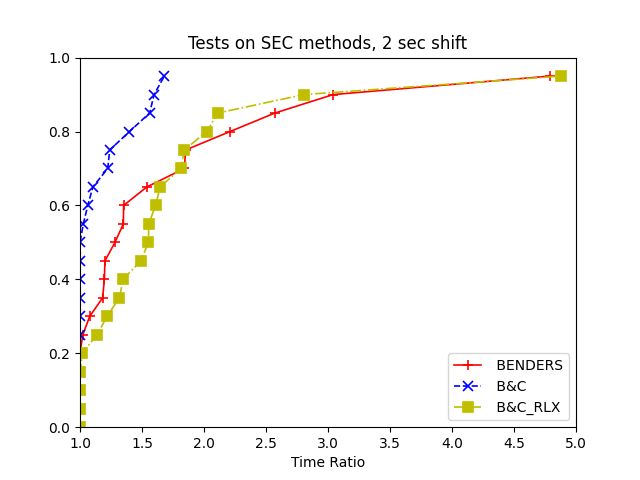
\includegraphics[width=0.6\textwidth]{images/final_SEC.png}
	\caption{The comparison chart of the SEC methods.}
	\label{fig:result-sec}
\end{figure}

The results in figure \ref{fig:result-sec} showed clearly that the Branch and Cut method is the best approach of this comparison. The most outstanding outcome is that the B\&C (Branch-and-Cut) relaxation method was in a trailing position even compared with the Benders method, while I was assuming that its performance was comparable with the normal B\&C.

The meaning of this is the fact that the callback is applied each time a fractional solution is found. This suggests that it is called way more times than in the previous one and this leads to worse performance. For solving this problem, I have done deeper research on this approach. Figure \ref{fig:result-bac} shows the B\&C relaxation applied with a different probability.

\begin{figure}[h]
	\centering
	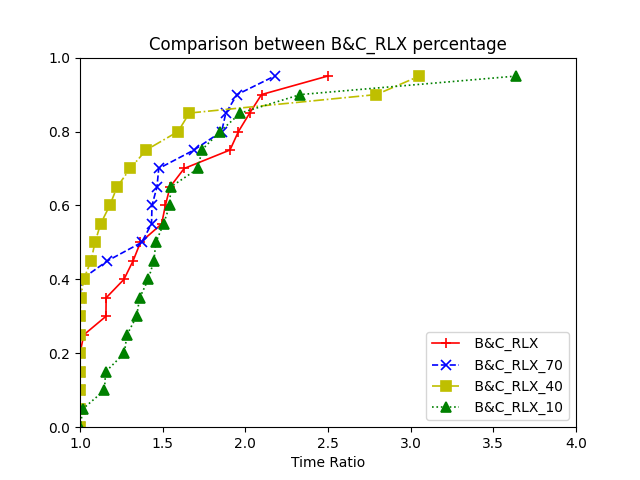
\includegraphics[width=0.6\textwidth]{images/branch_perc.png}
	\caption{The comparison between different B\&C relaxation.}
	\label{fig:result-bac}
\end{figure}

This plot shows that the best performing method is the one with a percentage of 40\%. In this way is possible to obtain the final chart with the best methods.

\begin{figure}[h]
	\centering
	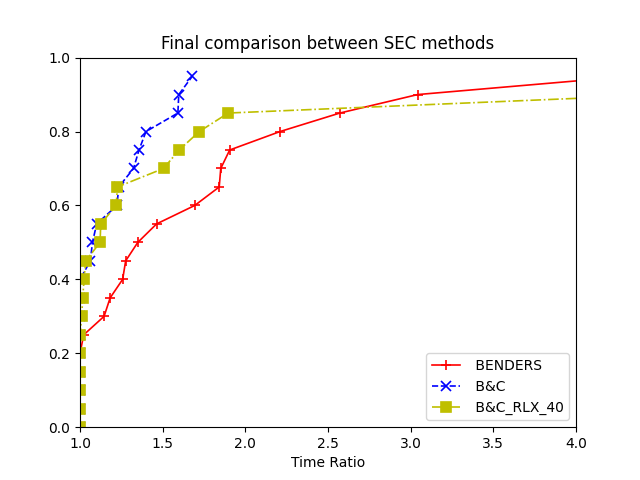
\includegraphics[width=0.6\textwidth]{images/final_final_SEC.png}
	\caption{Final comparison between different B\&C.}
	\label{fig:result-final-bac}
\end{figure}

This last chart shows that the classic Branch and Cut method and the relaxation one applied with a percentage of 40\% are similar, but the one that solves only the integer solution is considered the best among them.

